% AVD612 report - AI-assisted TECHNICAL DRAFT for the 3-member student team.
% Instructor policy: authors must review, verify, and rewrite in their own words.
% Replace author names/affiliations and confirm each result before Moodle submission.
\documentclass[conference,10pt]{IEEEtran}
\usepackage{amsmath,amssymb,graphicx,booktabs,cite,url}
\usepackage[T1]{fontenc}
\usepackage{microtype}
\graphicspath{{../results/simulation_graphs/}}
\newcommand{\vect}[1]{\mathbf{#1}}
\begin{document}
\title{Simulation and Evaluation of an LMS Adaptive Equalizer\\for BPSK and QPSK Communication Links}
\author{\IEEEauthorblockN{Team Member 1 \quad Team Member 2 \quad Team Member 3}
\IEEEauthorblockA{Department / Institute (replace), AVD612 Course Project\\
Email addresses / instructor details (replace)}}
\maketitle
\begin{abstract}
A least-mean-squares (LMS) adaptive equalizer is studied in a reproducible Python model of a symbol-spaced digital link. A finite impulse response (FIR) dispersive channel introduces inter-symbol interference (ISI), and additive white Gaussian noise (AWGN) perturbs the received symbols. A known training sequence updates the equalizer coefficients; weights are frozen before evaluating new, held-out symbols. Both real-valued binary phase-shift keying (BPSK) and complex-valued quadrature phase-shift keying (QPSK) are supported using one complex-correct LMS routine. At 12 dB measured receive-signal SNR on the chosen three-tap channel, the BPSK bit-error rate (BER) reduces from 0.1549 without equalization to 0.0217 after equalization, while QPSK reduces from 0.1591 to 0.0247. Experiments also explore learning rate, filter length, channel severity, convergence, and error-vector magnitude (EVM). The implementation demonstrates both the usefulness and limitations of a training-based linear equalizer.
\end{abstract}
\begin{IEEEkeywords}
Adaptive filter, LMS, channel equalization, inter-symbol interference, BPSK, QPSK, Python.
\end{IEEEkeywords}

\section{Introduction}
Digital symbols transmitted through channels with memory are smeared across adjacent symbol times. The resulting inter-symbol interference (ISI) causes a receiver to make errors even when thermal noise is small. An equalizer counters the channel memory by filtering the received samples before symbol decisions. Fixed filters require a known and stable channel; adaptive equalizers instead estimate suitable filter coefficients from observed signals \cite{proakis2007,haykin2002}. Their usefulness extends to wired links, radio baseband receivers, and communication demonstrations.

The subsystem considered here is a \emph{training-based linear LMS equalizer}. The project implements a single-spaced complex-capable transversal FIR filter in Python and tests the filter using BPSK and QPSK, as well as varied signal-to-noise ratios (SNRs), channel impulse responses, step sizes, and numbers of taps. The goal is to study \emph{equalization}, not modulation classification or carrier/timing recovery. GNU Radio's Linear Equalizer and Adaptive Algorithm provide related design patterns, although no GNU Radio implementation is copied here \cite{gnuradioeq,gnuradioadaptive}.

\section{Informal Operation of the Subsystem}
A transmitter maps random information bits onto unit-power BPSK ($\pm 1$) or QPSK ($\{\pm1\pm j\}/\sqrt{2}$) symbols. A three-tap channel adds delayed copies of the current symbols, followed by AWGN. For the main experiment, the channel response is $h=[0.90,\ 0.65,\ -0.35]$, intentionally creating substantial ISI.

The equalizer takes the current and $M-1$ previous received samples and forms a weighted sum. During a preamble, the transmitter's symbols are known to the receiver, making it possible to compute a training error. The LMS rule updates weights toward a smaller instantaneous squared error. A decision delay $D$ compensates for causal filtering. After the training window the weights are \emph{frozen}; the receiver then makes hard decisions on unseen symbols. The known test bits are consulted only \emph{after} this process to measure BER. This prevents ground-truth test leakage and isolates equalizer performance.

\section{Mathematical Model and Derivation}
\subsection{Communication Channel and Linear Filter}
With transmitted symbol $s[n]$, channel taps $h[\ell]$, and independent zero-mean AWGN $v[n]$, the received complex baseband signal is
\begin{equation}
 r[n]=\sum_{\ell=0}^{L_h-1}h[\ell]s[n-\ell]+v[n].
 \label{eq:channel}
\end{equation}
The instantaneous equalizer input, coefficient vector, and output are
\begin{align}
 \vect{x}[n]&=[r[n],r[n-1],\ldots,r[n-M+1]]^T,\\
 \vect{w}[n]&=[w_0[n],\ldots,w_{M-1}[n]]^T,\\
 y[n]&=\vect{w}^H[n]\vect{x}[n]. \label{eq:output}
\end{align}
The desired signal is $d[n]=s[n-D]$. Defining
\begin{equation}
 e[n]=d[n]-y[n], \qquad J(\vect{w})=E\{|e[n]|^2\},
 \label{eq:err}
\end{equation}
leads to the Wiener mean-square objective, the same optimization principle used in adaptive filtering \cite{widrow1985,haykin2002}.

\subsection{From Wiener--Hopf to Stochastic Gradient}
For stationary data, let $\vect{R}=E\{\vect{x}\vect{x}^H\}$ and $\vect{p}=E\{\vect{x}d^*\}$. Expanding the mean-square error,
\begin{equation}
 J(\vect{w})=\sigma_d^2-\vect{w}^H\vect{p}-\vect{p}^H\vect{w}
       +\vect{w}^H\vect{R}\vect{w}.
\end{equation}
Taking the complex gradient with respect to $\vect{w}^*$ gives $\partial J/\partial\vect{w}^*=\vect{R}\vect{w}-\vect{p}$. Thus, the minimizer satisfies the Wiener--Hopf equations
\begin{equation}
 \vect{R}\vect{w}_{\mathrm{opt}}=\vect{p},\qquad
 \vect{w}_{\mathrm{opt}}=\vect{R}^{-1}\vect{p},
 \label{eq:wiener}
\end{equation}
when $\vect{R}$ is nonsingular. LMS avoids forming $\vect{R}$, estimating $\vect{p}$, and inverting a matrix at each update. Instead it replaces the expected gradient by its instantaneous counterpart $-\vect{x}[n]e^*[n]$, yielding
\begin{equation}
 \boxed{\vect{w}[n+1]=\vect{w}[n]+\mu\vect{x}[n]e^*[n].}
 \label{eq:lms}
\end{equation}
Here $\mu>0$ is the step size. The conjugation is essential for complex QPSK and is implicit for real-valued BPSK. In the code, $\vect{w}^H\vect{x}$ is evaluated using \texttt{np.vdot(w, x)}. One common idealized mean-convergence guide is $0<\mu<2/\lambda_{\max}(\vect{R})$; finite-sample mean-square stability is more restrictive and depends on input statistics \cite{haykin2002}. Large $\mu$ generally adapts faster initially but can have greater residual error or instability.

\subsection{Evaluation Metrics}
For $N_b$ held-out bits, the measured bit-error rate is
\begin{equation}
 \mathrm{BER}=\frac{1}{N_b}\sum_{i=1}^{N_b}\mathbb{I}\{\hat b_i\ne b_i\}.
\end{equation}
With complex symbol estimates $\hat s_k$ and known references $s_k$, the measured root-mean-square error-vector magnitude is
\begin{equation}
 \mathrm{EVM}_{\mathrm{RMS}}=\sqrt{\frac{\sum_k|\hat s_k-s_k|^2}{\sum_k|s_k|^2}}.
\end{equation}
Test EVM and test BER evaluate the same held-out symbol indices. The \emph{unequalized} comparator uses raw $r[k]$ for symbol $s[k]$, while the equalizer uses $y[k+D]$ for the same $s[k]$.

\section{Python Simulation and Methodology}
The simulator uses a reproducible pseudorandom bit sequence, unit-average-energy symbols, discrete-time convolution with $h$, and AWGN of variance set from the \emph{measured power of the noiseless received signal}. This SNR convention is explicitly signal-power SNR, not $E_b/N_0$. Both a real channel and a real-valued BPSK receiver or complex-valued QPSK receiver can be simulated. Coefficients are initialized to zero.

Unless otherwise specified, the FIR equalizer has $M=9$ taps, step size $\mu=0.018$, delay $D=2$, $2500$ training time samples, and $9000$ evaluated test symbols; the main test uses SNR $=12$ dB. The first $M-1$ samples have no full input window and are excluded from coefficient updates. The test symbols do not appear in the adaptation targets, and the weight vector is held constant during evaluation. Fixed seeds permit exact regeneration; the SNR sweep averages three separate seeds. No results in this report are from a physical radio.

\section{Simulation Results and Discussion}
\subsection{Baseline Improvement}
Table~\ref{tab:main} reports a single representative seed (2026). The equalizer significantly reduces BER and EVM in the modeled dispersive link at 12 dB. The improved QPSK constellation in Fig.~\ref{fig:constellation} is consistent with ISI mitigation; residual spread remains due to AWGN and imperfect finite-length equalization.
\begin{table}[!t]
\centering\caption{Measured held-out performance at 12 dB (seed 2026).}
\label{tab:main}
\begin{tabular}{@{}llrr@{}}\toprule
Modulation & Metric & Without LMS & With LMS \\ \midrule
BPSK & BER & 0.1549 & 0.0217 \\
BPSK & RMS EVM & 0.7924 & 0.4550 \\
QPSK & BER & 0.1591 & 0.0247 \\
QPSK & RMS EVM & 0.7950 & 0.4592 \\ \bottomrule
\end{tabular}
\end{table}
\begin{figure}[!t]
\centering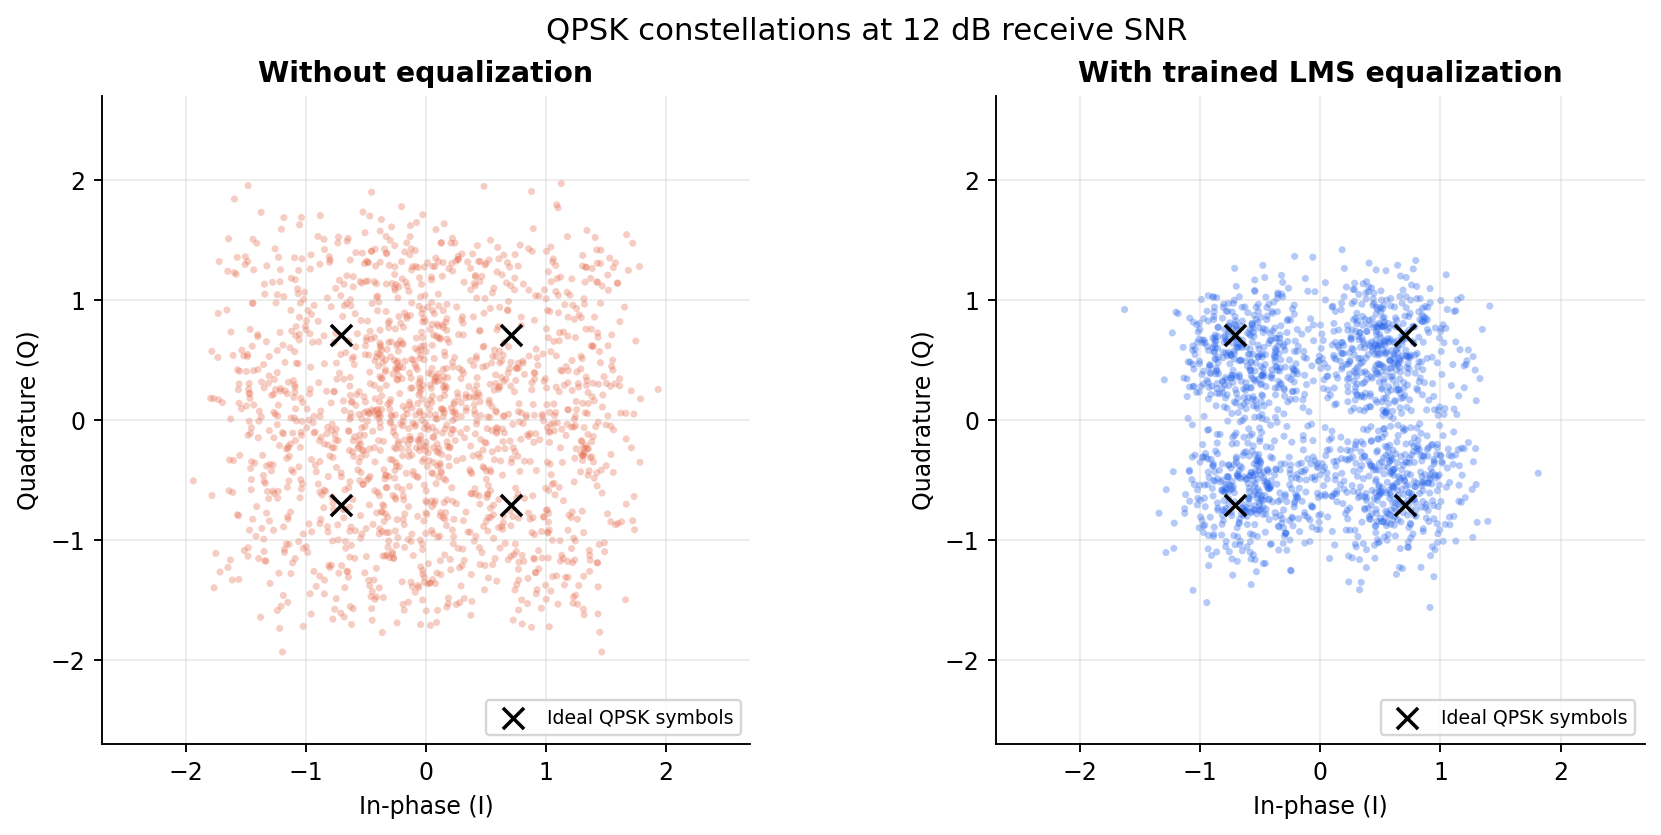
\includegraphics[width=\columnwidth]{02_qpsk_constellation.png}
\caption{QPSK received constellation, before and after LMS, compared with ideal points.}
\label{fig:constellation}
\end{figure}
\begin{figure}[!t]
\centering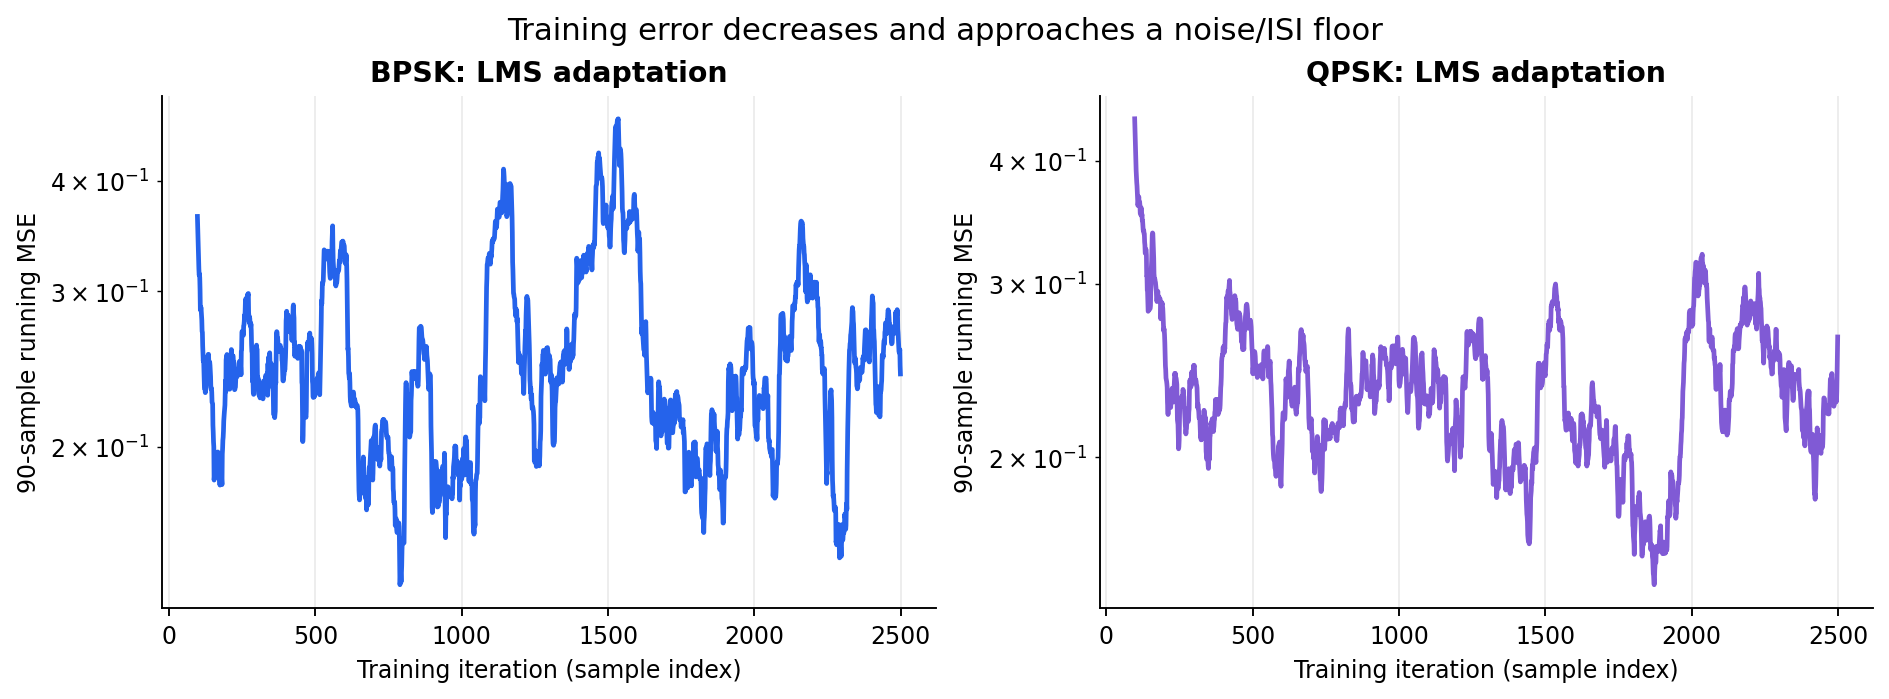
\includegraphics[width=\columnwidth]{01_mse_convergence.png}
\caption{Running training MSE for BPSK and QPSK. Learning reduces the error but does not remove AWGN or all ISI.}
\label{fig:mse}
\end{figure}

\subsection{Learning Rate, Filter Length, and SNR}
The training-MSE curves in Fig.~\ref{fig:mse} show a decreasing mean-square error during adaptation. Figure~\ref{fig:mu} compares four step sizes. In this particular channel and training interval, $\mu=0.004$ gives test BER $\approx0.0171$, whereas $\mu=0.07$ yields $\approx0.0599$, demonstrating that faster, larger updates do not necessarily provide better steady-state detection. A separate tap sweep uses $M\in\{3,5,9,13,17\}$: BER reaches $\approx0.0217$ at nine taps, with no consistent improvement at larger tap counts. These are case-specific numerical observations, not universal optimal settings. Figure~\ref{fig:taps} visualizes the filter-length tradeoff for this experiment.
\begin{figure}[!t]
\centering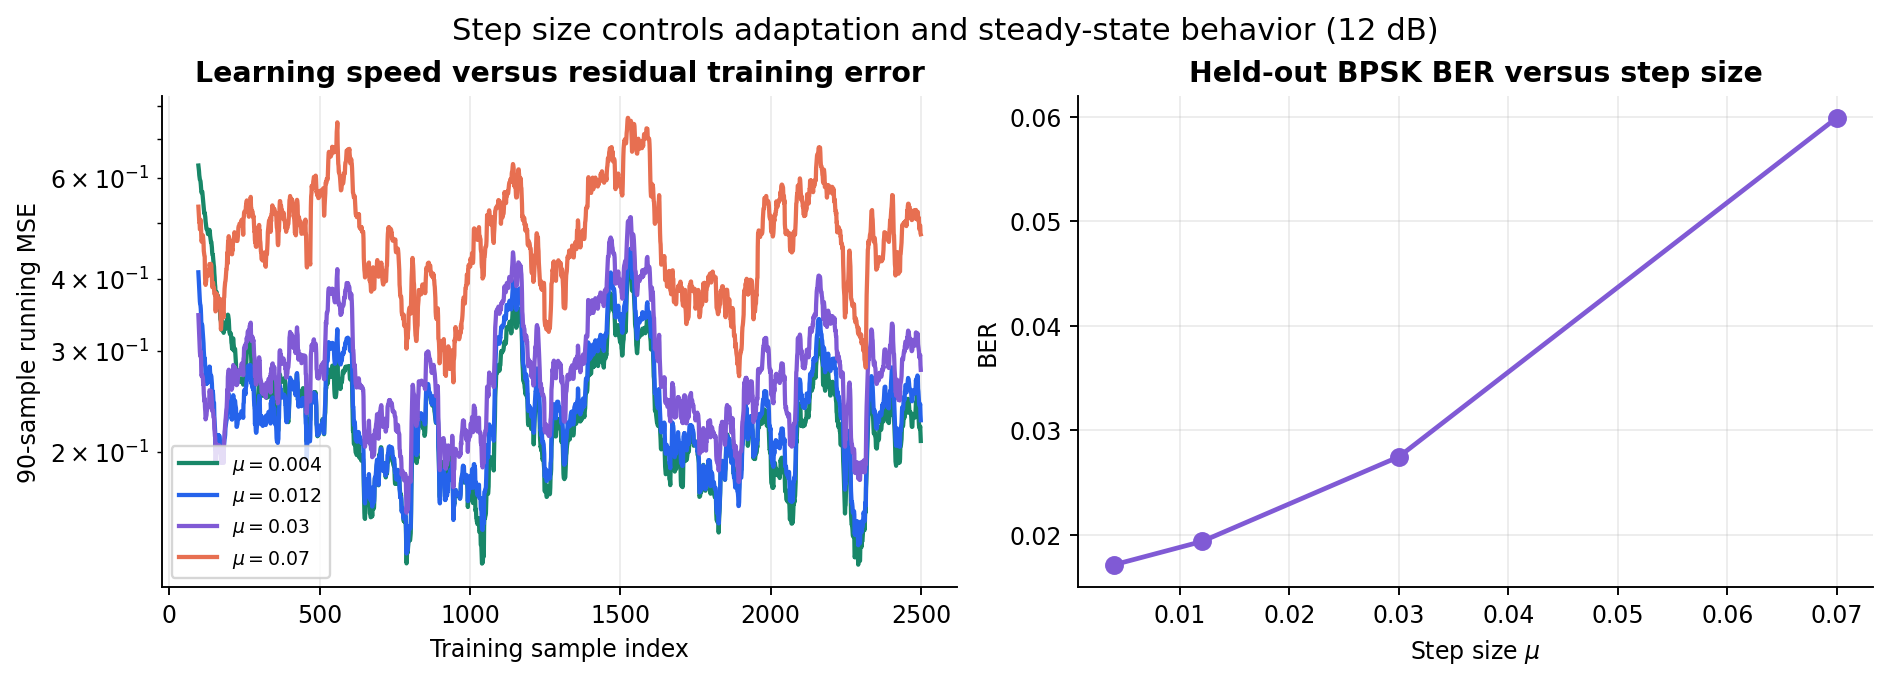
\includegraphics[width=\columnwidth]{04_stepsize_sweep.png}
\caption{Effects of the LMS learning rate on training error and held-out BPSK BER at 12 dB.}
\label{fig:mu}
\end{figure}
\begin{figure}[!t]
\centering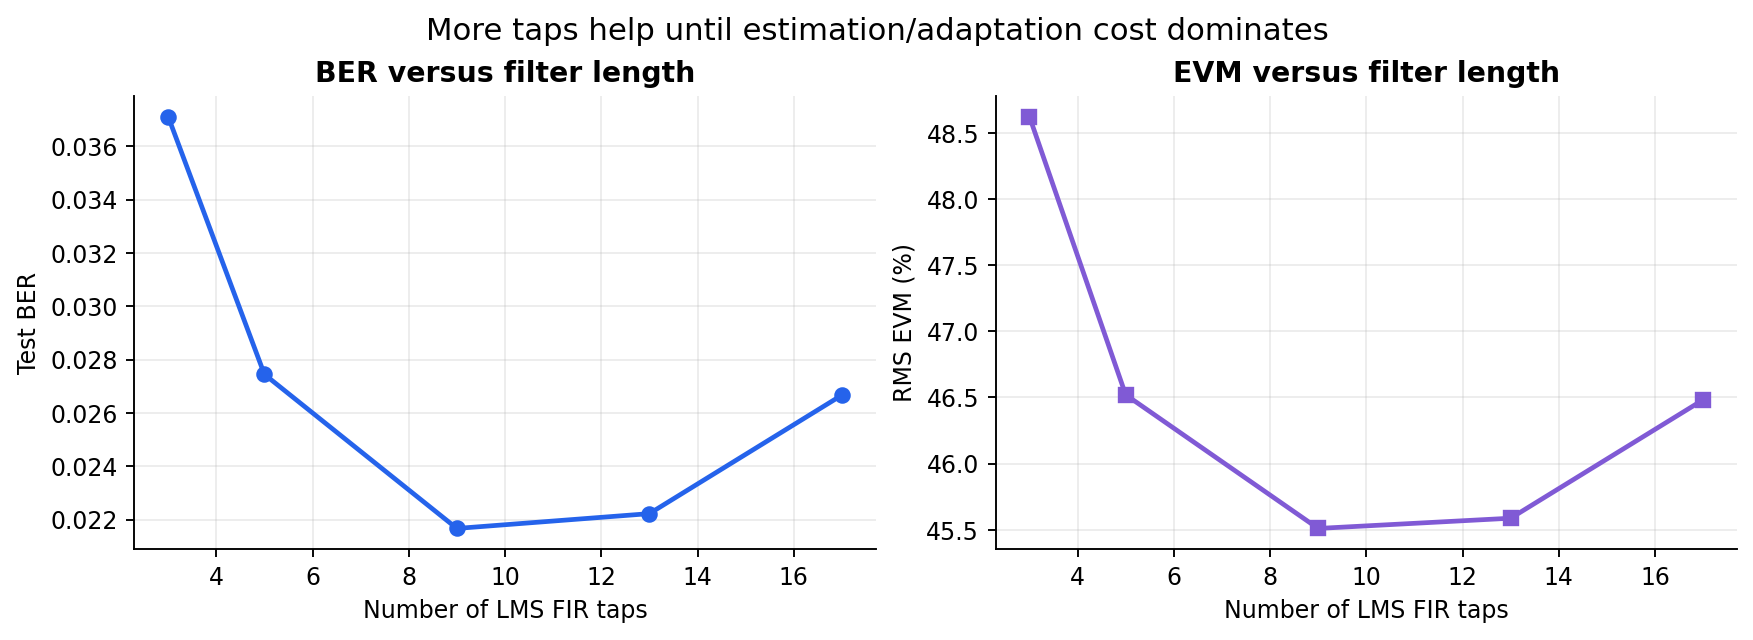
\includegraphics[width=\columnwidth]{05_filter_length_sweep.png}
\caption{Held-out BPSK BER and RMS EVM as the FIR equalizer tap count varies.}
\label{fig:taps}
\end{figure}
\begin{figure}[!t]
\centering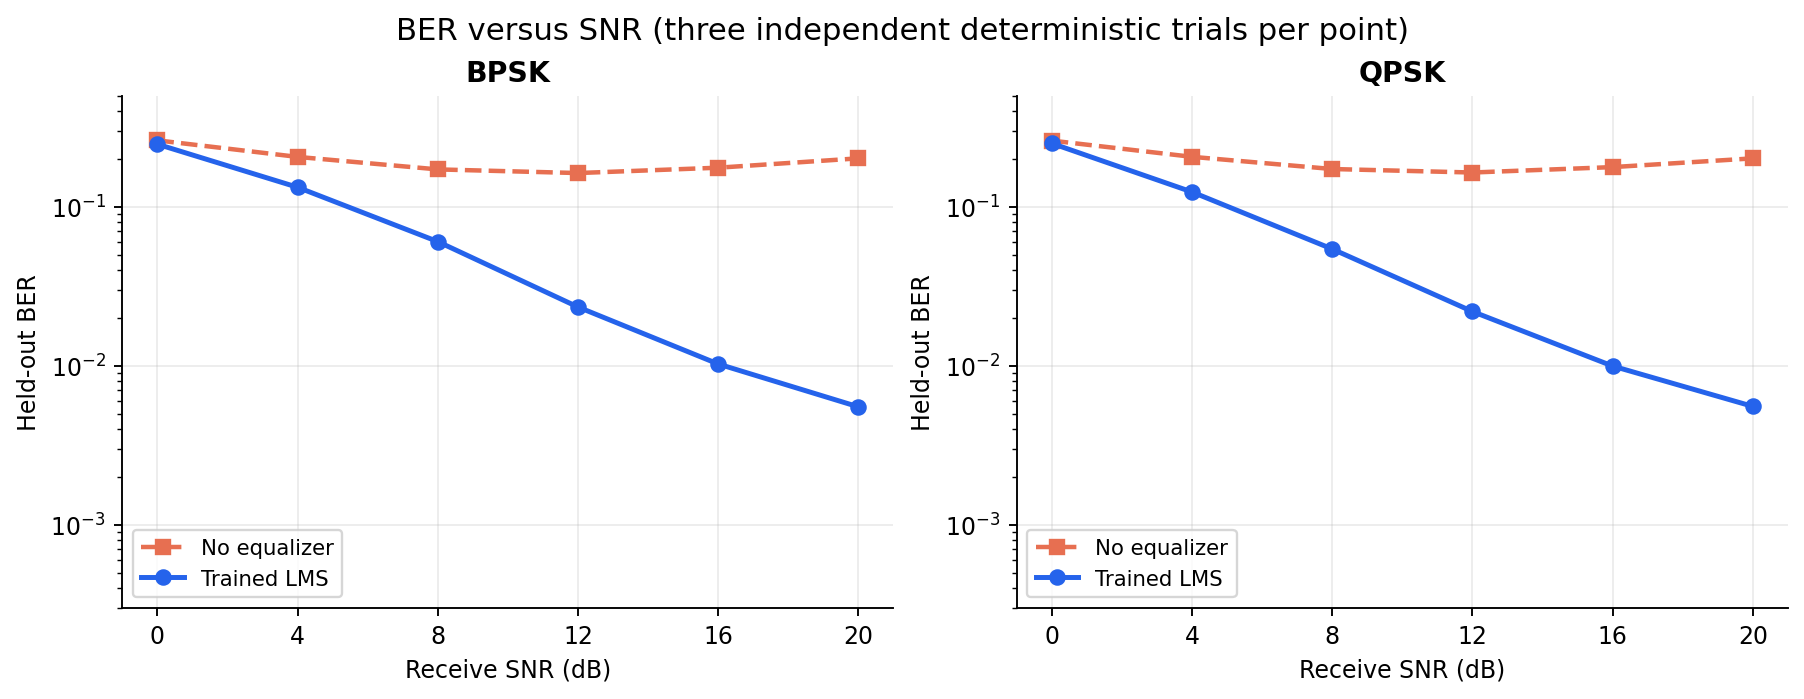
\includegraphics[width=\columnwidth]{06_ber_vs_snr.png}
\caption{BER versus signal-power SNR: average of three independent seeded simulations at each SNR.}
\label{fig:ber}
\end{figure}

Figure~\ref{fig:ber} gives the held-out BER across 0--20 dB. The LMS equalizer improves performance substantially over much of the SNR range but is not guaranteed to do so at the noisiest settings. The raw channel has an \emph{ISI-driven error floor}; because the interferer can dominate a symbol, modest extra noise can sometimes shift hard decisions in either direction, so raw BER need not decrease monotonically for a fixed severe ISI channel. It would be incorrect to describe these curves as textbook AWGN-only BER.

\subsection{Additional Tests and Reproducibility}
The package includes waveform comparisons, learned-coefficient trajectories, effective channel--equalizer impulse responses, filter-length sweeps, and a three-channel comparison (flat, mild, severe). The combined impulse response $g=h*\overline{\vect{w}}$ (Fig.~\ref{fig:imp}) has its largest desirable component near delay $D$. A short equalizer can leave ISI around the desired delay; a longer one raises complexity and can enhance noise.
\begin{figure}[!t]
\centering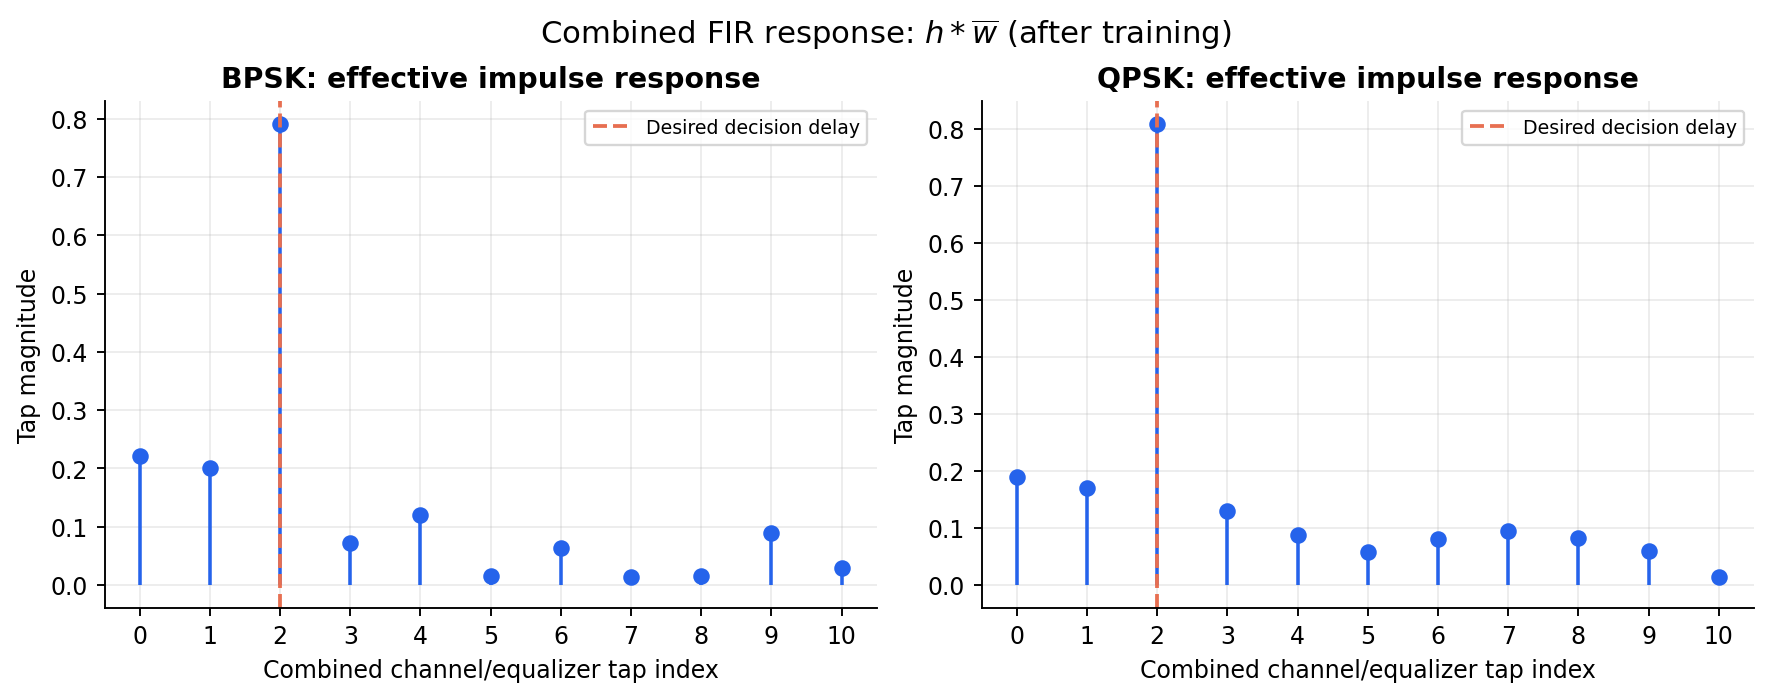
\includegraphics[width=\columnwidth]{07_effective_impulse_response.png}
\caption{Magnitude of effective channel-plus-equalizer impulse response; dashed marker indicates desired delay.}
\label{fig:imp}
\end{figure}
Source code, executable notebook, machine-readable metrics, and unit tests allow the figures and measurements to be reproduced. The flat-channel test also serves as a limiting case: if ISI is absent, adaptation has little scope to improve an already good link.

\section{Limitations and Conclusion}
This simulator assumes symbol synchronization, phase alignment, a stationary FIR channel, ideal availability of training symbols, and hard-decision detection. It omits pulse-shaping, carrier and timing recovery, fading mobility, pilot overhead, and decision-directed adaptation. In particular, a conventional eye diagram would require oversampled samples; none is asserted from the symbol-spaced data here.

A correctly aligned, training-only LMS equalizer reduces ISI and improves BER and EVM for both BPSK and QPSK in the chosen test link. Step size and FIR length involve measurable tradeoffs; there is no universal parameter choice. Future work could extend the setup to measured channels, normalized LMS, time-varying taps, and decision-directed operation.

\bibliographystyle{IEEEtran}
\bibliography{references}
\end{document}
